\documentclass[a4paper,12pt]{article}
\usepackage[ngerman]{babel}
\usepackage{ucs}
\usepackage{multirow}
\usepackage{xltxtra}
\usepackage[utf8x]{inputenc}
\usepackage{fontspec}
\usepackage{eurosym}
\usepackage{graphicx}
\usepackage[paper=a4paper,left=25mm,right=25mm,top=25mm,bottom=25mm]{geometry}
\usepackage{makecell}
\usepackage[table]{xcolor}
\usepackage{float}
\usepackage[normalem]{ulem}
\usepackage{xcolor,colortbl}
\definecolor{Gray}{gray}{0.85}
\usepackage[automark]{scrlayer-scrpage}
\usepackage[
	colorlinks=true,
	urlcolor=blue,
	linkcolor=green
]{hyperref}
\usepackage{float}
\restylefloat{table}
\setlength{\parindent}{0em}
\setlength{\parskip}{1ex}
\pagestyle{scrheadings}
\clearscrheadfoot
\setmainfont[Mapping=tex-text]{Liberation Serif}
\begin{document}
\input{theme.tex}
\input{version.tex}
\ohead{Last edit: \commitDate, id: \commitID}
\title{\tagYear\ Cyberspace Challenges Rules}
\makeatletter
\let\inserttitle\@title
\makeatother
\begin{center}
	\rrcybLogo
	\huge                      % Schriftgröße einstellen
	\bfseries                   % Fettdruck einschalten
	\\
	\inserttitle
\end{center}

\section{General Information}

\begin{center}
\emph{"`Fun while Learning, Sharing, Teamwork"'} despite Covid-19 -
\\
\textbf{RoboRAVE Germany goes Cyberspace!}
\end{center}

RoboRAVE Cyberspace is the online competition of RoboRAVE Germany.

We have expanded the
\href{https://www.roberta-home.de/lab/}{Open Roberta Lab}
and developed new challenges especially for RoboRAVE Cyberspace.
Equip your robot model with sensors and program it to find its way around new
tracks in the 2D simulation.

Here you will find the most recent RoboRAVE Cyberspace Challenges
\href{https://cyberspace.roborave.de}{cyberspace.roborave.de}.

Depending on the challenge, the tracks will not be published for scoring until
the day of the competition.

\subsection{Rules of Play}

\begin{itemize}
	\item Each team can submit one solution per hour, which will be played
		for scoring by the organisers in their simulation and - if
		possible - streamed live.
	\item The behaviour of the simulation depends on the hardware of the
		computer.  Teams should be prepared to engineer around this
		technical condition.
	\item Depending on the challenge, the robot has a certain number of
		minutes to complete the tasks.
	\item If the robot gets stuck in the simulation, i.e. if no progress
		can be observed for several seconds, the run may be aborted
		by the organisers. The organisers decide when to abort the run.
		In the case of an abort, the achieved partial points are taken
		into account, but not the remaining time.
\end{itemize}

\subsection{Divisions}

The teams of the RoboRAVE Cyberspace Challenges compete in different divisions:

\begin{itemize}
	\item ES – Elementary School: below 10 years of age
	\item MS – Middle School: 10 - 13 years of age
	\item HS – High School: 14 - 20 years of age
\end{itemize}

In RoboRAVE Cyberspace the teams may choose the division regardless of their
actual age. Each team must commit to a single division for RoboRAVE Cyberspace,
which then applies to all challenges. The division determines the difficulty
and the prize money to be won.

\subsection{Scoring}

The total score is the sum of the points from:
\begin{itemize}
	\item Completing the track to the respective destination. The tracks
		are divided into sections. For each completed section there are
		sub-points as indicated in the point tables of the challenges.
	\item Remaining time in seconds. A certain time is set for each
		challenge. If the track is completed to the finish before this
		time has elapsed, the remaining seconds are added to the total
		score.
\end{itemize}

\section{Line Following Challenge}

\subsection{Goal}

Configure and program a line-following robot that can follow a black line on a
white background to a "`tower"' (TOWER) within two minutes and then return to
its starting point (HOME).

\subsection{The Track}

\begin{itemize}
	\item Tracks for practising are available at
\href{https://cyberspace.roborave.de}{cyberspace.roborave.de}
	\item Division ES – no intersection, 1,25 cm black line
	\item Division MS – one intersection, 1,25 cm black line
	\item Division HS – two intersections, 0,75 cm black line
	\item A new design is created each year.
	\item There will be a minimum of 20 cm of straight line leading into
		the tower.
	\item Home and Tower are marked by a colour-coded rectangular obstacle.
	\item The line will be no closer than 10 cm from the edge of the track
		or any other line.
	\item Advertisement, or printed instructions can be placed anywhere on
		the track surface, but must be a minimum of 10cm from any line
	\item Curves can have different/changing radiuses, but no part of the
		curve can have a radius less than 15cm for ES \& MS, and 10cm
		for HS divisions.
\end{itemize}

\begin{center}
\begin{table}[H]
	\begin{tabular}{|c|c|c|} \hline
		ES & MS & HS \\
		\hline
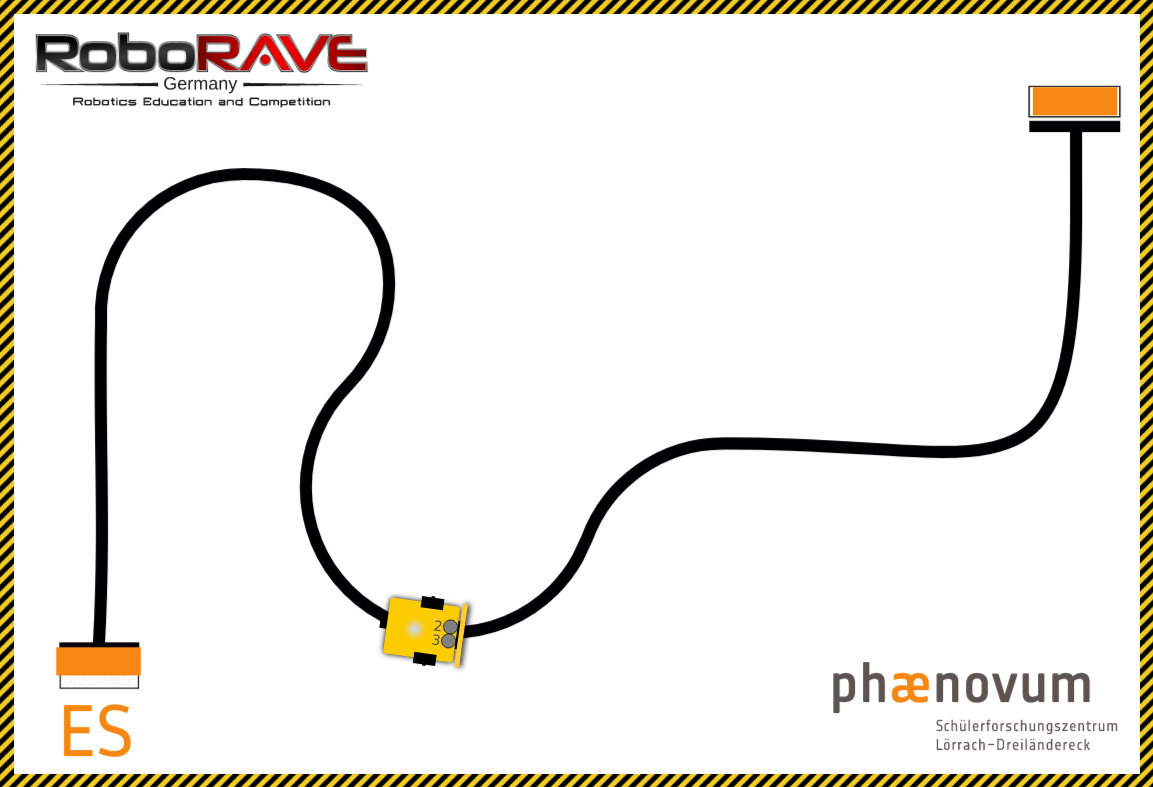
\includegraphics[width=0.3\textwidth]{images/cyberspace/linefollowing_es.png}
&
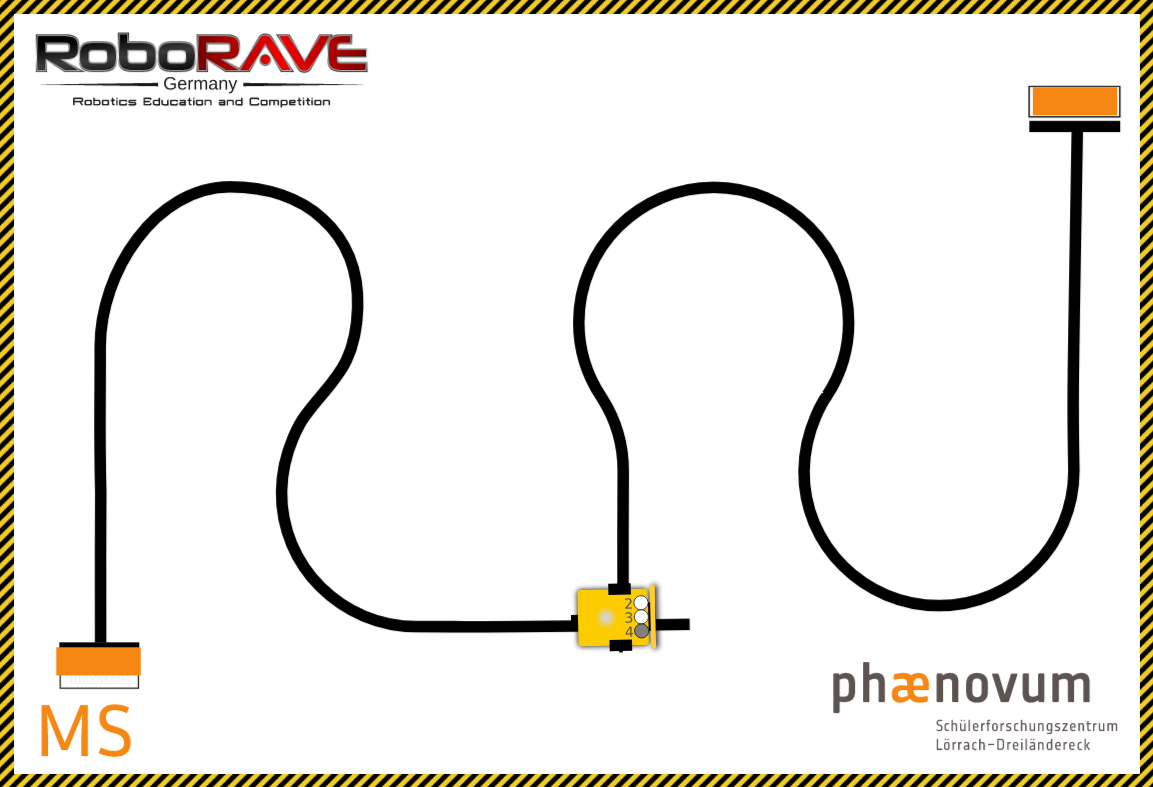
\includegraphics[width=0.3\textwidth]{images/cyberspace/linefollowing_ms.png}
&
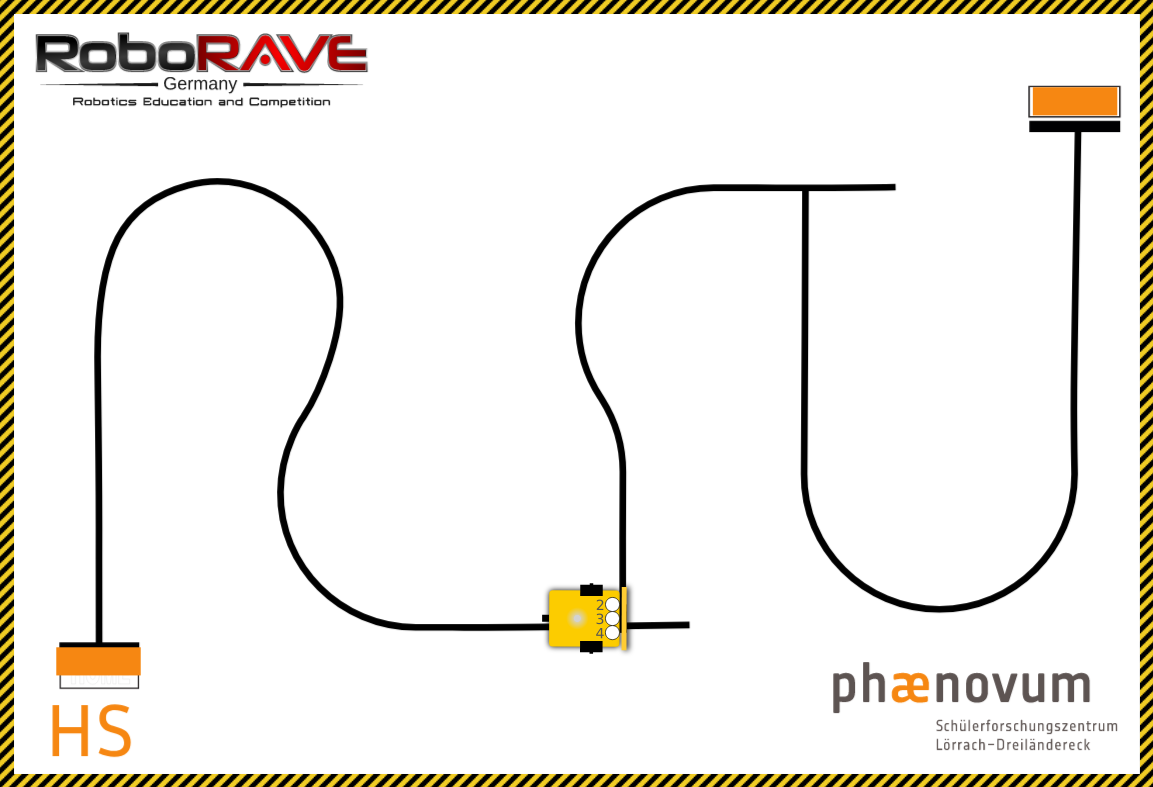
\includegraphics[width=0.3\textwidth]{images/cyberspace/linefollowing_hs.png}
\\
    		\hline
	\end{tabular}
\caption{\label{tab:table-name}Track Examples.}
\end{table}
\end{center}

\emph{Tracks shown are an \textbf{example}. The design changes every year and
are revealed on the first day of an event.}

\subsection{Scoring}

Scores according to the scoring table plus remaining time in seconds.
\begin{center}
	\begin{tabular}{|c|c|c|c|c|c|} \hline
		\multirow{3}*{} & Leaves & Passes 1st & Passes 2nd & Stops at \\
		& Home & Intersection & Intersection & Tower \\ \hline
		ES & 50 & n/a & n/a & 100 \\ \hline
		MS & 25 & 25 & n/a & 100 \\ \hline
		HS & 25 & 25 & 25 & 50 \\ \hline
	\end{tabular}
	\begin{tabular}{|c|c|c|c|c|c|} \hline
		\multirow{3}*{} & Starts Back & Passes 1st & Passes 2nd & Returns & Total \\
		& Home & Intersection & Intersection & Home &  \\ \hline
		ES & 50 & n/a & n/a & 100 & 400 \\ \hline
		MS & 25 & 25 & n/a & 100 & 400 \\ \hline
		HS & 25 & 25 & 25 & 100 & 400 \\ \hline
	\end{tabular}
\end{center}

\section{Labyrinth Challenge}

\subsection{Goal}

Configure and program a robot that can (in three minutes) find its way through
a maze of obstacles to its destination by means of sensors (not exclusively the
rotation sensors of the motors).

\subsection{The Track}

\begin{itemize}
	\item Tracks for practising are available at
\href{https://cyberspace.roborave.de}{cyberspace.roborave.de}
	\item Division ES – no dead end
	\item Division MS – one dead end
	\item Division HS – two dead ends
	\item A new design may be created each year.
	\item The corridors of the labyrinth are at least 20 cm wide
	\item The corners of the labyrinth are always rectangular, the walls
		are always horizontal or vertical.
	\item The goal is marked by a square obstacle highlighted in colour.
	\item Advertisement, or printed instructions can be placed anywhere on
		the track surface, but must be a minimum of 10cm from any line
\end{itemize}

\begin{center}
\begin{table}[H]
	\begin{tabular}{|c|c|c|} \hline
		ES & MS & HS \\
		\hline
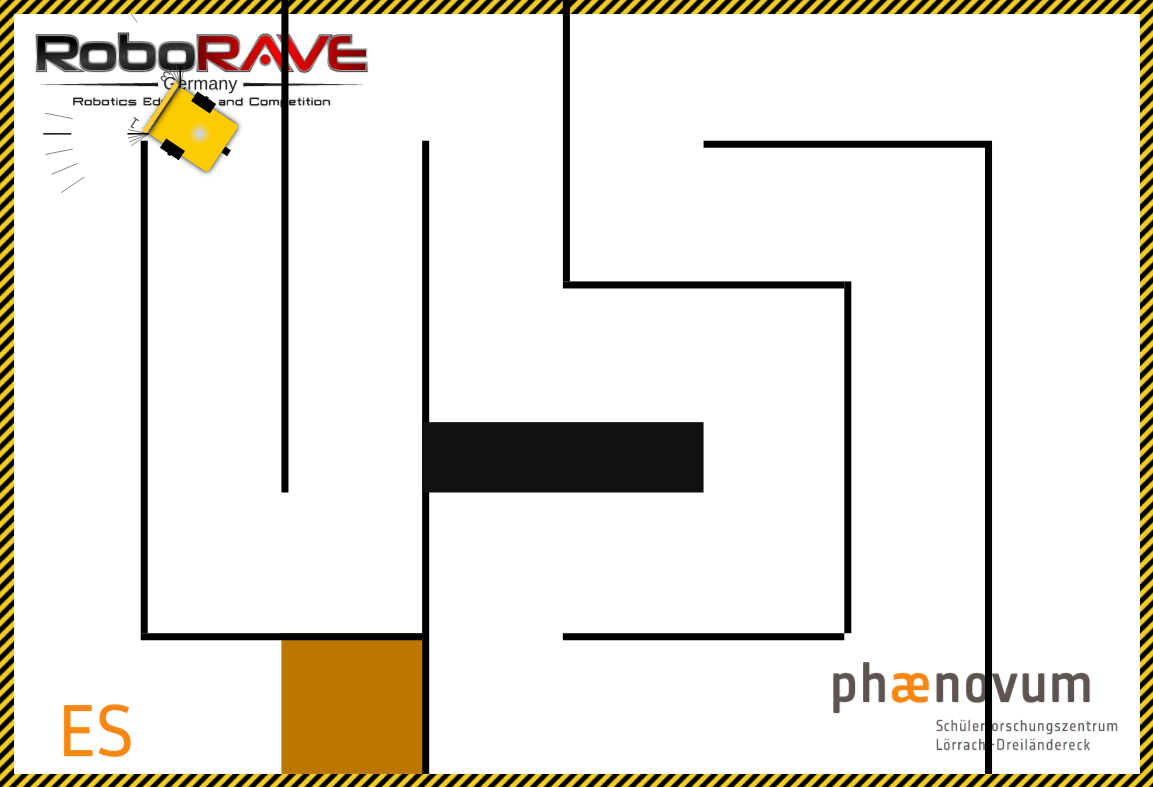
\includegraphics[width=0.3\textwidth]{images/cyberspace/labyrinth_es.png}
&
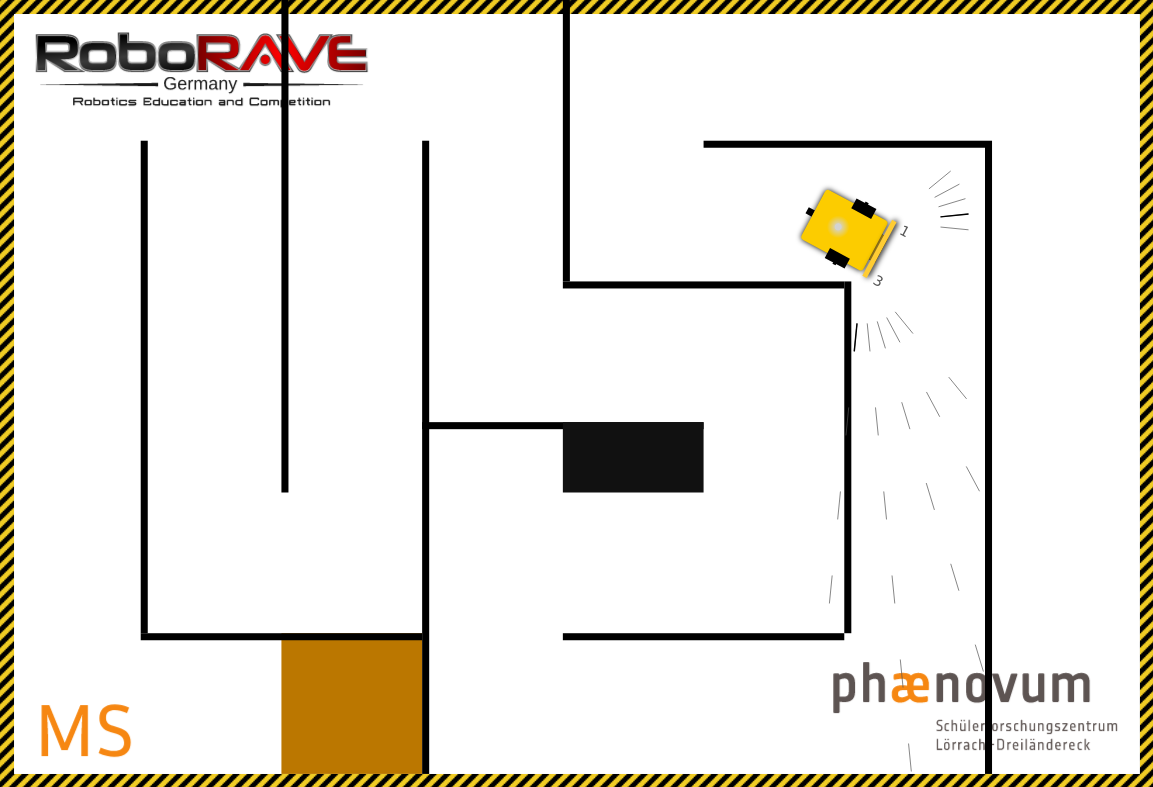
\includegraphics[width=0.3\textwidth]{images/cyberspace/labyrinth_ms.png}
&
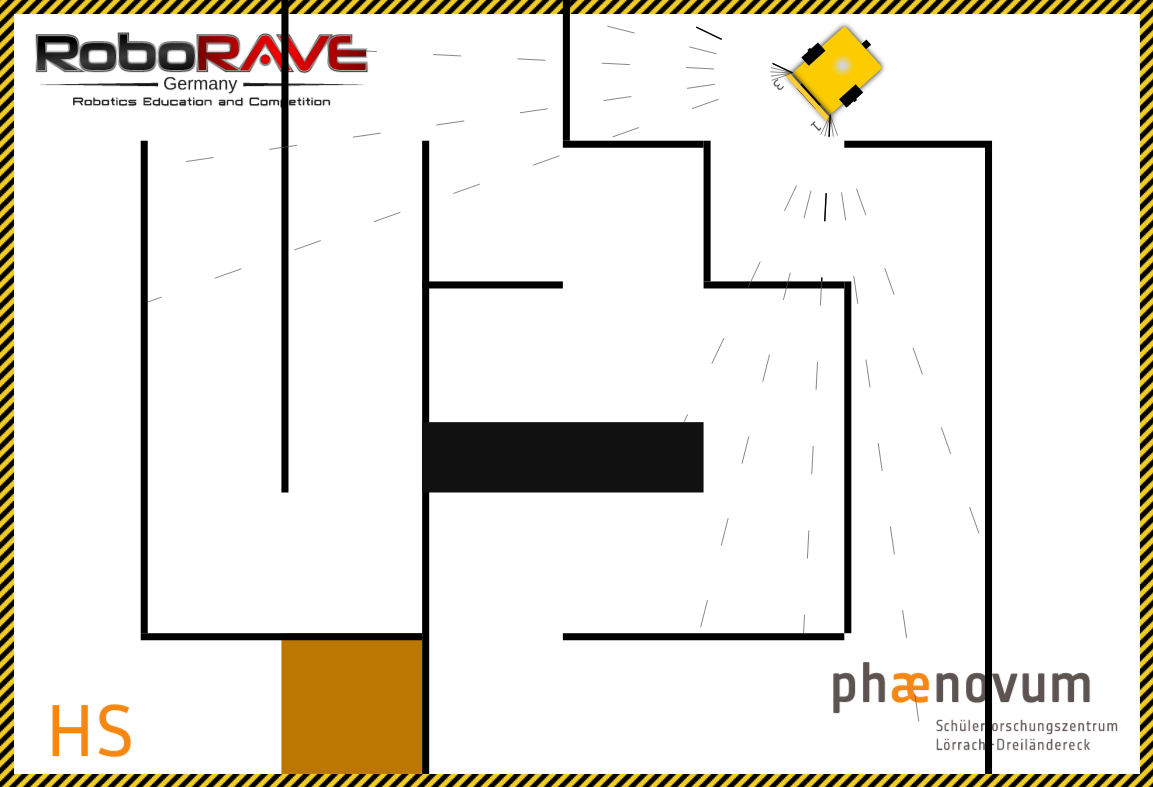
\includegraphics[width=0.3\textwidth]{images/cyberspace/labyrinth_hs.png}
\\
    		\hline
	\end{tabular}
\caption{\label{tab:table-name}Track Examples.}
\end{table}
\end{center}

\emph{Tracks shown are an \textbf{example}. The design changes every year and
are revealed on the first day of an event.}

\subsection{Scoring}

10 points per aisle covered plus remaining time in seconds. An aisle is limited
by start, corner(s) or finish.

\section{Rainbow Challenge}

\subsection{Goal}

Configure and program a robot that detects (in five minutes) the coloured paths
by means of sensors and travels along them in the order of the colours of the
rainbow to the obstacle and back.

\subsection{The Track}

\begin{itemize}
	\item Tracks for practising are available at
\href{https://cyberspace.roborave.de}{cyberspace.roborave.de}
	\item Each path has a different colour.
	\item Division ES – 4 Paths, colour and shape of the paths do not
		change.
	\item Division MS – 4 paths, shape of the paths does not change, their
		colour is random.
	\item Division HS – 6 paths, shape of the paths does not change, their
		colour is random.
	\item Colour codes:
\begin{center}
	\begin{tabular}{|c|c|c|c|c|} \hline
		Farbe & RGB (Hexadecimal) & Red & Green & Blue \\ \hline
    		Red & e40303 & 228 & 3 & 3 \\
    		Orange & ff8c00 & 255 & 140 & 0 \\
    		Yellow & ffed00 & 255 & 237 & 0 \\
    		Green & 008026 & 0 & 128 & 38 \\
    		Blue & 004dff & 0 & 77 & 255 \\
    		Purple & 750787 & 117 & 7 & 135 \\ \hline
	\end{tabular}
\end{center}
	\item Division ES/MS – the paths can take the colours red, yellow,
		green and blue That is 24 possible combinations.

	\item Division HS – the paths can additionally take on the colours
		orange and purple. That is 720 possible combinations.
	\item The centre circle is surrounded by an edge, which is detected by
		the robot as grey and differs from the colours of the paths.
	\item Division ES/MS - the centre circle is filled black.
	\item Division HS - the centre circle is filled white.
	\item The background of the track does not contain the colours of the
		paths.
	\item Division ES/MS - the background of the track is detected as grey
		with white patterns by the colour sensor.
	\item Division HS - the background of the track is detected as black
		with grey patterns by the colour sensor.
	\item The end of the paths is marked by a rectangular obstacle
		highlighted in colour
	\item Division ES/MS - the path are about 10 cm wide
	\item Division HS - the path are about 5 cm wide
	\item Division ES/MS - the corners of the paths are always
		right-angled, the paths always run horizontally or vertically.
	\item Division HS - the corners of the paths can have any angle.
	\item Advertisements or printed instructions can be placed anywhere on
		the board, but not behind the paths
	\item A new design may be created each year.
\end{itemize}

\begin{center}
\begin{table}[H]
	\begin{tabular}{|c|c|c|} \hline
		ES & MS & HS \\
		\hline
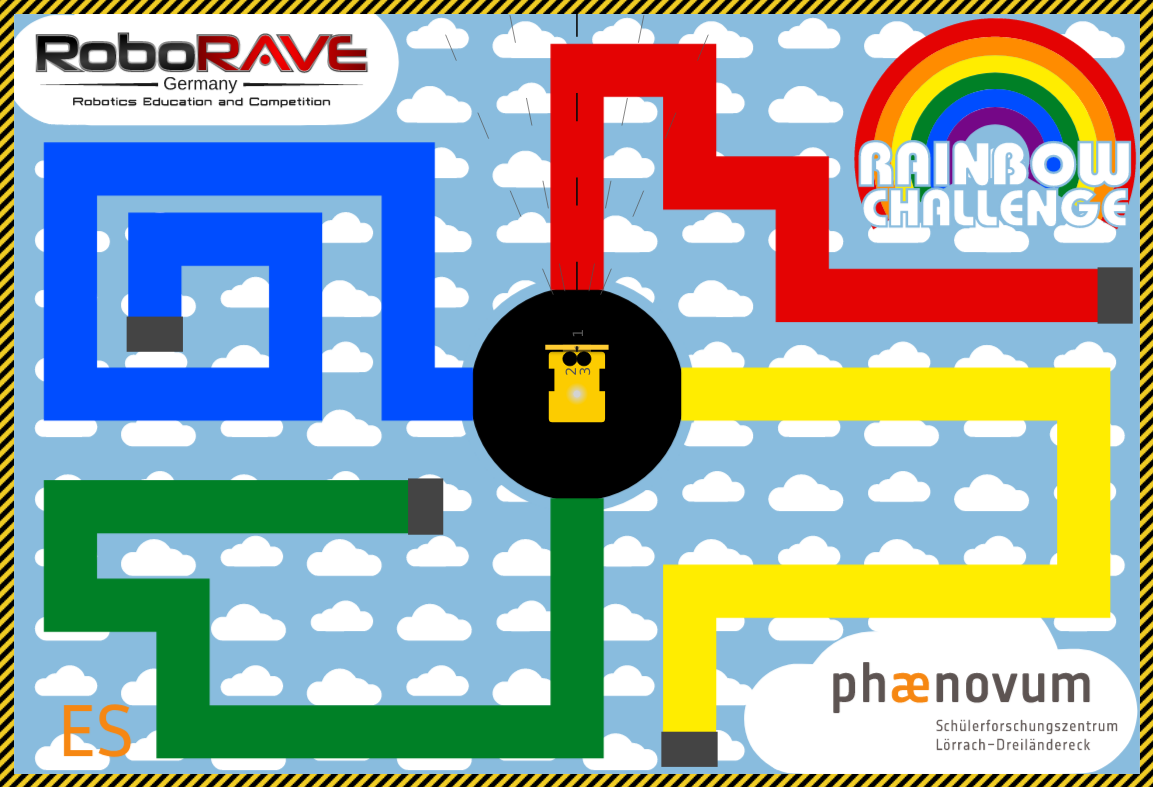
\includegraphics[width=0.3\textwidth]{images/cyberspace/rainbow_es.png}
&
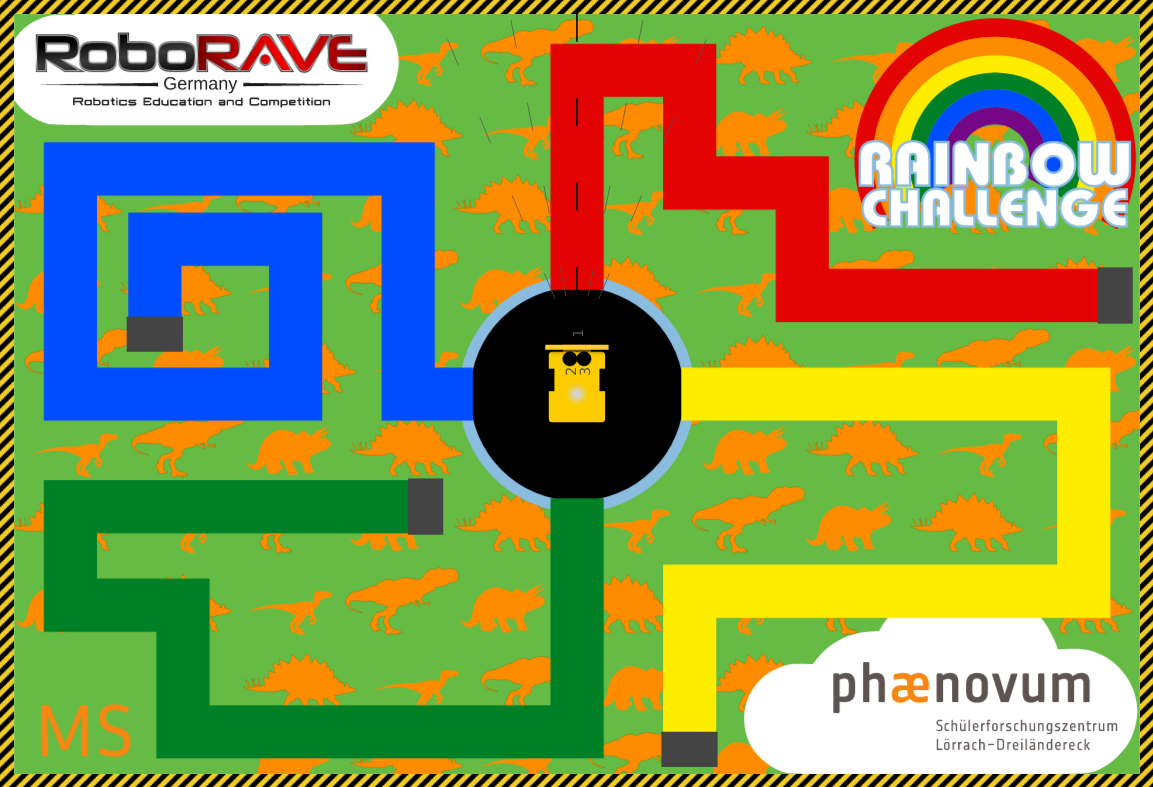
\includegraphics[width=0.3\textwidth]{images/cyberspace/rainbow_ms.png}
&
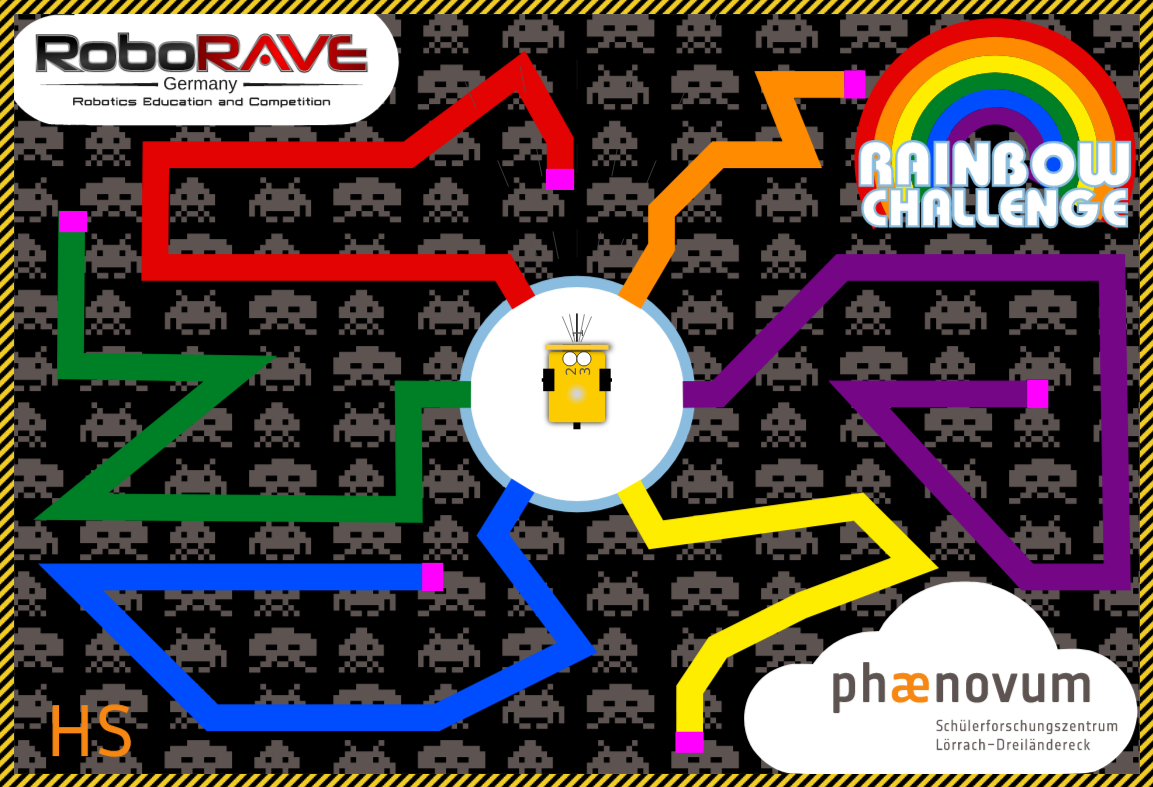
\includegraphics[width=0.3\textwidth]{images/cyberspace/rainbow_hs.png}
\\
    		\hline
	\end{tabular}
\caption{\label{tab:table-name}Track Examples.}
\end{table}
\end{center}

\subsection{Scoring}

For each start from the correct path 10 points, 10 more points for driving to
the end of the path and another 10 points for driving back to the centre
circle, plus remaining time in seconds.

\end{document}
